% !TEX root = ../YourName-Dissertation.tex

\chapter{Precise Analysis on Single-trace Attacks}\label{chapter4}

\section{Problem}
Side channels are ubiquitous in modern computer systems as sensitive
information can leak through many mechanisms such as power,
electromagnetic radiation, and even
sound~\cite{agrawal2002side,kar20178,chari1999towards,217605,genkin2014rsa}.
Among them, software side-channel attacks, such as cache attacks, memory page
attacks, and controlled-channel attacks, are especially problematic as they do not require physical proximity~\cite{7163052,217543,217589,lee2017inferring,191010,liu2015last}. These
attacks arises from shared micro-architectural components in a computer processor.
By observing inadvertent interactions between two programs, attackers can infer program
execution flows that manipulate secrets and guess secrets such as encryption
keys~\cite{Osvik2006,Gullasch:2011:CGB:2006077.2006784,203878,10.1007/978-3-540-45238-6_6}.


Recent work~\cite{203878,217537,Wichelmann:2018:MFF:3274694.3274741,Brotzman19Casym,236338,182946}
can detect many side-channel vulnerabilities. For example,
DATA~\cite{217537} reports 2,248 potential leakage sites for the RSA
implementation in OpenSSL 1.1.0f\@.
Further analysis shows 1,510 leaks can be dismissed. But that
leaves 460 data-access leaks and 278 control-flow leaks.
Many of these vulnerabilities have not been fixed by developers for a variety of reasons.
First, some vulnerable implementations perform better. For example,
RSA implementations usually adopt the CRT optimization,
which is faster but vulnerable to fault attacks~\cite{aumuller2002fault}.
Second, fixing vulnerabilities can introduce new
weaknesses.
Third, most vulnerabilities pose a negligible risk.
Although some vulnerabilities result in the key being
entirely compromised~\cite{184415, aumuller2002fault},
many others are less
severe in reality. Therefore, we need a proper quantification metric to
assess the sensitivity of side-channel vulnerabilities,
so a developer can efficiently triage them.

Previous work~\cite{182946,5207642} can identify numerous leakages or even provide an upper bound on the amount of leakage, which is useful to verify that an implementation is secure if it incurs zero leakage.
However, these techniques cannot quantify the severity of a leak because they over approximate the leakage. For example, CacheAudit~\cite{182946}
reports that the upper-bound leakage of AES-128 exceeds the original key size. Besides, existing side-channel quantification work~\cite{182946,5207642} assumes an attacker runs the target program multiple times with different
input secrets and calculates an ``average'' estimation, which is different from real attack scenarios when the secret that an attacker wants to retrieve is fixed. As a consequence, those results are less useful to assess the severity level of each leakage site.

To overcome these limitations, we propose a novel method to quantify information
leakage precisely. We quantify the number of bits that can leak during a real
execution and define the amount of leaked information as the cardinality of
possible secrets based on an attacker's observation. Before an attack, an adversary has a large but finite input space.
Whenever the adversary observes a leakage site, they can eliminate some impossible
inputs and reduce the input space's size. In an extreme case, if the input space's size reduces to one, an adversary has determined the input, which means all secret information (e.g., the entire secret key) is
leaked. By counting the number of inputs~\cite{10.1007/11499107_24}, we can quantify the information leakage precisely.
We use symbolic execution to generate constraints to model the relation
between the original sensitive input and an attacker's observations.
Symbolic execution provides fine-grained information, but it is expensive
to compute. Therefore, prior symbolic
execution work~\cite{203878,236338,Brotzman19Casym} either analyzes only
small programs or applies domain knowledge~\cite{203878} to simplify the analysis. We
examine the bottleneck of the trace-oriented symbolic execution and optimize it
to work for real-world crypto-systems.

We have implemented the proposed technique in a tool called \tool{} and demonstrated
it on real-world crypto libraries, including OpenSSL,
mbedTLS, Libgcrypt, and Monocypher.
We collect execution traces of these libraries and apply
symbolic execution to each instruction. We model
each side-channel leak as a logic formula. These
formulas precisely model side-channel vulnerabilities.
Then we use the conjunction of those formulas to model the
leaks at a statement that appears in different location in
the execution trace file (e.g., leaks inside a loop).
Finally, we introduce a Monte Carlo sampling method to estimate
the information leakage.
The experimental results confirm
that \tool{} precisely identifies previously known vulnerabilities and
reports how much information is leaked and which byte in the original sensitive
buffer is leaked. We also test \tool{} on side-channel-free algorithms.
\tool{} produces no false positives.
The result also shows the newer version of crypto libraries leak less information
than earlier versions.
\tool{} also discovers new vulnerabilities. With the help of \tool{},
we confirm that some of these vulnerabilities are severe.


%Based on the fixed attack target, we classify the software-based side-channel
%vulnerabilities into two categories: 1.\textit{secret-dependent control-flow
%transfers} and 2.\textit{secret-dependent data accesses} and model them with
%math formulas which constrain the value of sensitive information. We quantify
%the amount of leaked information as the number of possible solutions that are
%reduced after applying each constrains.


%Our method can identify and quantify address-based sensitive information
%leakage sites in real-world applications automatically. Adversaries can exploit
%different control-flow transfers and data-access patterns when the program
%processes different sensitive data. We refer them as the potential information
%leakage sites. Our tool can discover and estimate those potential information
%leakage sites as well as how many bits they can leak. We are also able to
%report precisely how many bits can be leaked in total if an attacker observes
%more than one site. We run symbolic execution on execution traces. We model
%each side-channel leakage as a math formula. The sensitive input is divided
%into several independent bytes and each byte is regarded as a unique symbol.
%Those formulas can precisely model every the side-channel vulnerability. In
%other words, if the application has a different sensitive input but still
%satisfies the formula, the code can still leak the same information.  
%Those information leakage sites may spread in the whole program and their
%leakages may not be dependent. Simply adding them up can only get a coarse
%upper bound estimate. In order to accurately calculate the total information
%leakage, we must know the dependent relationships among those multiple leakages
%sites. Therefore, we introduce a monte carlo sampling method to estimate the
%total information leakage.

In summary, we make the following contributions:

\begin{itemize}
    \item We propose a novel method that can quantify fine-grained leaked
          information from side-channel vulnerabilities that result from actual attack
          scenarios. Our approach differs from previous ones in that we
          model real attack scenarios for one execution.
          We model the information quantification problem as a counting problem
          and use a Monte Carlo sampling method to estimate the information leakage.

    \item We implement the method into a tool and apply it
          to several pieces of real software. \tool{} successfully identifies
          previous unknown and known side-channel vulnerabilities and calculates the corresponding information leakage.
          Our results are useful in practice.
          The leakage estimates and the corresponding trigger inputs can
          help developers to triage and fix the vulnerabilities.
\end{itemize}

\section{Threat Model}

The threat model is similar to our previous work. That is, we assume
an attacker can share some hardware resource with the victim. The attacker has
the ability to probe the victim at any time of the execution. We also assume
an attacker has noise-free observations. The attacker has the access to the victim's
binary executable. The threat mode is similar to
the previous work~\cite{203878,182946,Brotzman19Casym} and can catch most of
the address-based side-channel attacks in the literature.


\section{Background}
Given an event $e$ that occurs with the probability $p(e)$, we receive
\begin{displaymath}
    I = - \log_2p(e)
\end{displaymath}
bits of information by knowing the event $e$ happens according to information theory~\cite{shannon1948mathematical}.
Considering a char variable $a$
with one byte storage size in a C program, its value ranges from 0 to 255.
Assume $a$ has a uniform distribution. If we observe that
$a$ equals $1$, the probability of this observation is $\frac{1}{256}$. So
we get $-\log(\frac{1}{256}) = 8$ bits information, which is exactly the size
of a char variable in the C program.

Existing works on information leakage quantification typically use Shannon
entropy~\cite{clark2007static,Wichelmann:2018:MFF:3274694.3274741},
min-entropy~\cite{10.1007/978-3-642-00596-1_21}, and max-entropy~\cite{182946,
    Doychev:2017:RAS:3062341.3062388}. In these frameworks, the input sensitive
information $K$ is considered as a random variable.

Let $k$ be one of the possible
value of $K$. The Shannon entropy $H(K)$ is defined as
\begin{displaymath}
    H(K) = - \sum_{k {\in} K}p(k)\log_2(p(k))
\end{displaymath}

Shannon entropy can be used to quantify the initial uncertainty about the
sensitive information. It measures the amount of information in a system.

Min-entropy describes the information leaks for a program with the most likely input.
For example, min-entropy can be used to describe the
best chance of success in guessing one's password using the
most common password. %, which is defined as
\begin{displaymath}
    \mathit{min\text{-}entropy} = - \log_2(p_{\mathit{max}})
\end{displaymath}

Max-entropy is defined solely on the number of possible observations.
%It is equal to $-\log_2{n}$.
\begin{displaymath}
    \mathit{max\text{-}entropy} = -\log_2{n}
\end{displaymath}
As it is easy to compute, most recent works~\cite{182946,Doychev:2017:RAS:3062341.3062388} use max-entropy as the definition of
the amount of leaked information.

To illustrate how these definitions work, we consider the code
fragment in Figure~\ref{fig:side-channel}. It has two secret-dependent
control-flows, A and B.

\begin{figure}[h!]
    \centering
    \begin{lstlisting}[xleftmargin=.2\textwidth, xrightmargin=.2\textwidth]
uint8_t key[2], t1, t2;
get_key(key);              // 0 <= key[0], key[1] < 256
t1 = key[0] + key[1];
t2 = key[0] - key[1];
if (t1 < 4){               // leakage site A
    foo();    
}                          
if (t2 > 0){               // leakage site B     
    doo();    
}                          
\end{lstlisting}
    \vspace*{-1pt}
    \caption{Side-channel leakage}
    \label{fig:side-channel}
\end{figure}
In this paper we assume an attacker can observe the secret-dependent control-flows in Figure~\ref{fig:side-channel}.
Therefore, an attacker can have two different observations for each leak site
depending on the value of the $\mathit{key}$: $A$ for function \textsf{foo} is executed,
$\neg A$ for function \textsf{foo} is not executed, $B$ for function \textsf{doo} is
executed, and $\neg B$ for function \textsf{doo} is not executed. Now the
question is how much information can be leaked from the above code if an
attacker knows which branch is executed?

\begin{table}[ht]
    \centering\small\footnotesize
    \caption{The distribution of observation}\label{shtable}
    %    \resizebox{\columnwidth}{!}{
    \begin{tabular}{l|cc|cc}
        \hline

        Observation ($o$)   & $A$    & $\neg A$ & $B$   & $\neg B$ \\ \hline
        Number of Solutions & 65526  & 10       & 32768 & 32768    \\ \hline
        Possibility (p)     & 0.9998 & 0.0002   & 0.5   & 0.5      \\
        \hline
    \end{tabular}
    %        }
\end{table}

Assuming $\mathit{key}$ is uniformly distributed, we can calculate the corresponding
possibility by counting the number of possible inputs. Table~\ref{shtable}
describes the probability of each observation. We use the above three types of
leakage metrics to calculate the amount of leaked information for leak A and leak B.

\textbf{Min Entropy.}
As $p_{A\mathit{max}} = 0.9998$ and $p_{B\mathit{max}} = 0.5$,
with the definition, min-entropy equals to
\begin{align*}
    \mathit{min\text{-}entropy_A} & = -\log_2{0.9998} = 0.000\ \mathrm{bits} \\
    \mathit{min\text{-}entropy_B} & = -\log_2{0.5} = 1.000\ \mathrm{bits}
\end{align*}

\textbf{Max Entropy.}
Depending on the value of key, the code can run two different branches for each leakage site.
Therefore, with the max entropy
definition, both leakage sites leak

\begin{displaymath}
    \mathit{max\text{-}entropy} = -\log_2{2} = 1.000\ \mathrm{bits}
\end{displaymath}

\textbf{Shannon Entropy.}
Based on Shannon entropy, the respective amount of information in A and B equals to
    {\footnotesize
        \begin{align*}
            \mathit{Shannon\text{-}entropy_A} & = -(0.9998*\log_{2}0.9998      \\
                                              & \qquad+ 0.0002*\log_{2}0.0002) \\
                                              & = 0.000\ \mathrm{bits}         \\
            \mathit{Shannon\text{-}entropy_B} & = -(0.5*\log_{2}0.5            \\
                                              & \qquad+ 0.5*\log_{2}0.5)       \\
                                              & = 1.000\ \mathrm{bits}
        \end{align*}
    }
In the next section, we will show that these measures work well only
theoretically in a static analysis setting.
Generally, they do not apply to dynamic analysis or real
settings. We will present that the static or theoretical results could be
dramatically different from the real world, and we do need a better method to
quantify the information leakage from a practical point of view.

\section{Leakage Definition}

In this section, we discuss how \tool{} quantifies the amount of leaked
information. We first present the limitation of existing quantification metrics.
Then, we introduce our model, the mathematical notation used in the
paper, and our method.

\subsection{Problem Setting}
Existing static side-channel quantification
works~\cite{182946,Wichelmann:2018:MFF:3274694.3274741,zhang2010sidebuster,bang2016string} define information
leakage using max entropy or Shannon entropy.  If zero bits of
information leakage is reported, a program is secure. However, when a tool using these metrics reports leakage, it is the ``average'' leakage. In a real attack, the leakage could be dramatically different.

\begin{figure}[h!]
    \centering
    \begin{lstlisting}[xleftmargin=.2\textwidth, xrightmargin=.2\textwidth]
char key[9] = input();
if(strcmp(key, "password"))   // leakage site C
    pass();                   // branch 1
else
    fail();                   // branch 2
\end{lstlisting}
    \vspace*{-10pt}
    \caption{A dummy password checker}
    \label{fig:password-checker}
\end{figure}

Consider a password checker sketched in Figure~\ref{fig:password-checker}.
The password checker takes an 8-byte char array (exclude \textsf{NULL} character)
and checks if the input is the correct password. If an attacker uses a side-channel attack to determine that the code executes branch
$\{{1\}}$, they can infer the password equals to
``password'', in which case the attacker retrieves the full password.
Therefore, the total leaked information should be 64 bits, which equals to the
size of the original sensitive input when the code executes branch
$1$.

However, prior static approaches cannot precisely capture the amount of leakage. According to the definition of Shannon entropy, the leakage will be
$\frac{1}{2^{64}}*\log_{2}\frac{1}{2^{64}} + \frac{2^{64}-1}{2^{64}}
    *\log_{2}\frac{2^{64}-1}{2^{64}} \approx 0$ bits. Max-entropy is defined from the
number of possible observations. Because the program has two
branches, tools based on max-entropy will report the code has a $\log_2{2} = 1$
bit leakage.
Both approaches fail to tell how much information is leaked during the execution
precisely. The problem with existing methods is that they are static-based so
input values and real runtime information are neglected by their approaches.
They assume an attacker runs
the program multiple times with many different or random sensitive inputs. As
shown in Figure~\ref{fig:gap}(a), previous models, both Shannon entropy and max
entropy, give an ``average'' estimate of the information leakage. However, it is
not the typical scenario for an adversary to launch a side-channel attack. When
a side-channel attack happens, the adversary wants to retrieve the sensitive
information, in which case the sensitive information is fixed (e.g., AES keys).
The adversary will run the attack over and over again with fixed input and
guess the value bit by
bit (e.g., Kocher's timing attacks~\cite{kocher1996timing}), as in Figure~\ref{fig:gap}(b). We want to have a
theory for dynamic analysis that if the theory says an attack leaks $x$ bits of
secret information from a side-channel vulnerability, then $x$ should be useful
in estimating the sensitive level of the vulnerability. However, the above
methods all fail in real attack models.
\begin{figure}
    \centering
    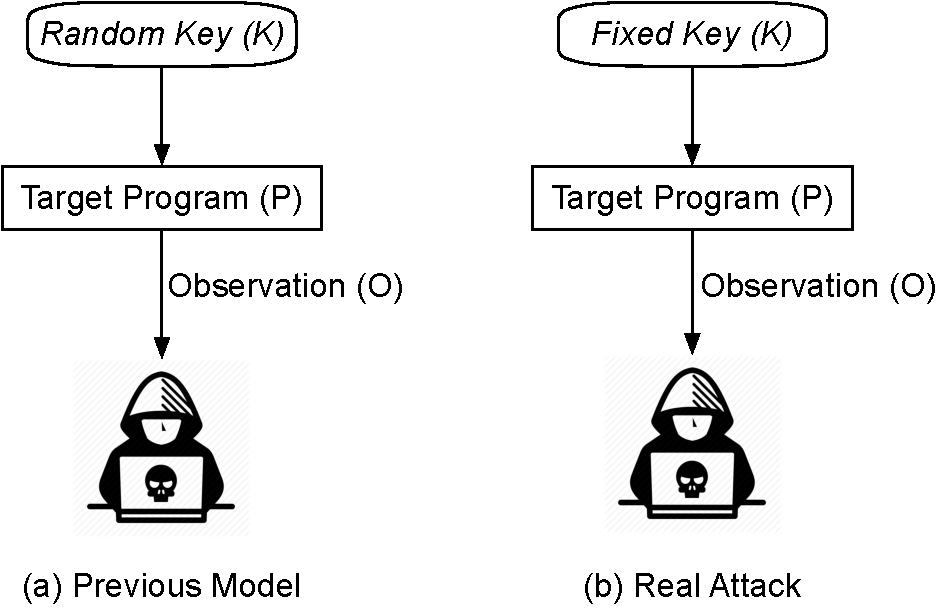
\includegraphics[width=.65\columnwidth]{./figures/chapter4/RA.pdf}
    \caption{The gap between the real attack and previous models}\label{fig:gap}
\end{figure}

\subsection{Precise Analysis}
Now we present our metric to quantify the amount of leaked information from
dynamic analysis.

We assume a program ($\beta$) has $K$ as its sensitive input. $K$ should be
a finite set of keys. The program also takes known messages $M$ as its input.
During an AES encryption, for example,
$\beta$ is the encryption function. $K$ is the set of all possible AES keys,
and $M$ represents the set consisting of all plaintext messages to be encrypted. In a real execution, an adversary may have
some observations ($O$) of the program. This paper only
uses secret-dependent control flows and secret-dependent data
accesses as observations.

With the above definition, we have the following mapping between $\beta$,
$K$, $M$, and $O$:
%\vspace*{-0pt}
\begin{displaymath}
    \beta(K, M) \rightarrow O
\end{displaymath}


We model a side-channel in the following way. An adversary does not have
access to $K$, but he knows $\beta$, $M$, and $O$. For one execution of a
deterministic program, once $k \in K$ and $m \in M$ are fixed, the observation
($o \in O$) should also be determined. An attacker knows $\beta$, $o$,
and $m$. The attacker wants to infer the value of $k$. We use $K^o$ to denote
the set of possible $k$ values that produce the same observation: $K^o = \{ k \in K \, |\, \beta(k, m) \rightarrow o\}$

Then the problem of quantifying the amount of leaked information can be
restated as the following question:

\emph{How much uncertainty of $K$ is reduced if an attacker knows $\beta$, $m$, and $o$?}

In information theory, the mutual information (I) is a measure of the mutual
dependence between two variables. Here we use I to describe the
dependence between original sensitive keys ($K$) and attackers' observations ($O$),
which is defined as:

\begin{equation} \label{eq:1}
    I(K;O) = \sum_{k {\in} K}{\sum_{o {\in} O}{p(k, o)\log_2\frac{p(k, o)}{p(k)p(o)}}}
\end{equation}

where $P(k_i, o_i)$ is the joint discrete distribution of $K$ and $O$.
Alternatively, the mutual information can also be equivalently expressed as:

\begin{equation} \label{eq:2}
    I(K;O) = H(K) - H(K|O)
\end{equation}

$H(K|O)$ is the entropy of $K$ with the condition $O$. It quantifies the
uncertainty of $K$ given the value of $O$. In other word, the conditional
entropy $H(K|O)$ marks the uncertainty about $K$ after an adversary has gained
some observations ($O$).
\begin{equation}
    H(K|O) = - \sum_{o {\in} O} {p(o) \sum_{k {\in} K}{p(k|o)\log_2p(k|o)}}
\end{equation}

In this project, we hope to give a very precise definition of information
leakages. Suppose an attacker runs the target program with one
fixed input, we want to know how much information he can infer by observing the
memory access patterns ($o$). We come to the simple slogan
~\cite{10.1007/978-3-642-00596-1_21} %% where the information
%% leakage equals:
%% \textbf{Initial uncertainty - remaining uncertainty}
that
\begin{align*}
     & \mathit{Information\ leakage} =                                       \\
     & ~~~~ \mathit{Initial\ uncertainty} - \mathit{Remaining\ uncertainty}.
\end{align*}

Next we compare the Eq.~(\ref{eq:2}) with the above slogan, we find $H(K)$
is the $\mathit{Initial\ uncertainty}$ and $H(K|O)$ is $\mathit{Remaining\
        uncertainty}$. During a real attack, the observation ($o$) is known.  Thus we
have $H(K|O) = H(K|o)$.

Therefore, we define the amount of leaked information as
\begin{displaymath}
    Leakage = H(K;o) = H(K) - H(K|o)
\end{displaymath}

For a program ($\beta$) without knowing any domain information, all possible sensitive
inputs should appear equally. Therefore, for any $k \in K$, $p(k) =
    \frac{1}{|K|}$. So we have
$$H(K) = \sum_{k {\in} K}\frac{1}{|K|}\log_2{|K|} = \log_2{|K|}$$
For any $k' \in K \setminus K^o$, $p(k'|o) = 0$. We get
\begin{align*}
    H(K;o) & = - \sum_{k {\in} K^o}{p(k|o)\log_2p(k|o)}                         \\
           & \qquad   - \sum_{k` {\in} (K \setminus K^o)}{p(k'|o)\log_2p(k'|o)} \\
           & = \sum_{k {\in} K^o}\frac{1}{|K^o|}\log_2{|K^o|}                   \\
           & = \log_2{|K^o|}
\end{align*}


\begin{mydef}
    \label{chatper4:def}
    Given a program $\beta$ with the input set $K$,
    an adversary has the observation $o$ when the input $k{\in}K^o$.
    We denote it as
    $$\beta(K^o, m) \rightarrow	o$$

    The amount of leaked information $L_{\beta(k)\rightarrow o}$ based on the observation ($o$) is
    $$L_{\beta(k)\rightarrow o} = \log_2{|K|} - \log_2{|K^o|}$$
\end{mydef}

The above definition~\cite{AskarovC12} can be understood in an intuitive way. Suppose an attacker
wants to guess a 128-bit encryption key from a program.
Without any domain knowledge,
he can find the key by performing exhaustive search over $2^{128}$ possible keys.
However, the program has a side-channel leakage site. After the program finishes execution, the
attacker get some leaked information and only need to find the key by performing
exhaustive search over $2^{120}$ possible keys. Then we can say that 8 bits of the information
is leaked. In this example, $2^{128}$ is the size of $K$ and $2^{120}$ is the size of $K^o$.


With the definition, if an attacker observes that the code in
Figure~\ref{fig:password-checker} runs the branch 1, then the $K^{o^{1}} =
    \{\mathrm{``password"}\}$. Therefore, the information leakage $L_{P(k)=o^{1}} =
    \log_2{2^{64}} - \log_2{1} = 64$ bits, which means the key is totally leaked. If
the attacker observes the code hits branch 2, the leaked information is
$L_{P(k)=o^{2}} = \log_2{2^{64}} - \log_2{(2^{64}-1)} \approx 0$ bit.


We can also calculate the leaked information from the sample code in
Figure~\ref{fig:side-channel}. As the size of input sensitive information is
usually public. The problem of quantifying the leaked information has been
transferred into the problem of estimating the size of input key $|K^o|$ under
the condition $o \in O$. The result is shown in Table~\ref{shtable2}. We can see
that some branches (e.g., A) or traces leak much more information than some others.
Those kinds of branches can be vulnerable when an attacker's data is incorporate.
For example, the code will skip some of the calculation if the value is 0 in big
number multiplication.

In
contrast, an \emph{average} estimate based on random secret input information is around
1 bit, as shown in the previous section and Table~\ref{shtable}, is
not very useful in practice as an attacker is able to get much more leaked
information in some attack scenarios.

\begin{table}[ht]
    \centering\small\footnotesize
    \caption{New leakage modeling results}
    \label{shtable2}
    \vspace*{-9pt}
    %    \resizebox{\columnwidth}{!}{
    \begin{tabular}{l|cc|cc}
        \hline

        Observation ($o$)         & $A$   & $\neg A$ & $B$   & $\neg B$ \\ \hline
        Number of Solutions       & 65526 & 10       & 32768 & 32768    \\ \hline
        Leaked Information (bits) & 0.0   & 14.7     & 1.0   & 1.0      \\
        \hline
    \end{tabular}
\end{table}

\subsection{Model Leakages}
\section{Approximate Model Counting}
\label{MCreasons}
In the previous section, we propose an information leakage definition for
realistic attack scenarios to model two types of address-based side-channel
leakages and showed how to quantify them by calculating the number of input
keys ($K^o$) that satisfy the formulas. Intuitively, we can use
symbolic execution to capture math formulas and model counting
to obtain the number of satisfying input keys ($K^o$). However, preliminary
experiments showed that this approach was far too expensive to use with real-world
applications. In this section, we discuss the bottlenecks in
this approach and propose a practical solution.


According to Definition~\ref{chapter4:def} introduced in the previous section,
the problem of quantifying the amount of leaked information can be reduced to
the problem of computing the number of items in $K^o$. However, we find that while
there are various propositional model counters (e.g., \#SAT), they are not
sufficient scalable for production cryptosystem analysis.
there is no open source modulo theories counter (\#SMT) available.

One straightforward method approximating the number of solutions is based on Monte Carlo
sampling. However, the number of satisfying values could be exponentially small.
Consider the formula $f_i\equiv{k_1} = 1\land{k_2} = 2\land{k_3} = 3\land{k_4} =
    4$, where $k_1$, $k_2$, $k_3$, and $k_4$ each represents one byte in the
original sensitive input buffer, there is only one satisfying solution of total
$2^{32}$ possible values, which requires exponentially many samples to get a
tight bound. Monte Carlo method also suffers from the curse of dimensionality.
For example, the length of an RSA private key can be as long as 4096 bits. If we
take each byte (8 bits) in the original buffer as one symbol, the formula can
have as many as 512 symbols.

%\vspace*{2pt}
%\textbf{Our Solution to Challenge C3:}
We adopt multiple-step Monte Carlo sampling methods to count the number of
possible inputs that satisfy the logic formula groups. The key idea is to split
those constraints into several small formulas and sample them independently.
We will introduce the method in the following subsection.

\subsection{Information Leakage Estimation}

\newcommand{\addr}[1]{{l}_{#1}}
\renewcommand{\addr}[1]{{\gamma}_{#1}}
\renewcommand{\addr}[1]{{\zeta}_{#1}}
\renewcommand{\addr}[1]{{\xi}_{#1}}

In this section, we present the algorithm to calculate the information leakage
based on Definition~\ref{def} (\S\ref{sec:trace-qif}), answering to
\textbf{Challenge C3}.

\subsection{Problem Statement}
For each leakage site, we model it with a constraint using the
method presented in~\S\ref{side-channel:condition}. Suppose the address of the
leakage site is $\addr{i}$, we use $c_{\addr{i}}$ to denote the constraint
that models its side-channel leakage.
%For
%multiple leakage sites, we take the conjunction of those constraints to
%represent those leakage sites.

According to the Definition~\ref{def}, to calculate the amount of leaked
information, the key is to calculate the cardinality
of $K^o$. Suppose an attacker can observe $n$ leakage sites, and each leakage
site has the following constraints: $c_{\addr{1}}, c_{\addr{2}}, \ldots,
    c_{\addr{n}}$ respectively. The total leakage can be calculated from the constraint
$c_t({\addr{1}},{\addr{2}},\ldots,{\addr{n}}) = c_{\addr{1}} \land c_{\addr{2}}
    \land \ldots \land c_{\addr{n}}$.
The problem of estimating the total leaked
information can be reduced to the problem of counting the number of different
solutions that satisfies the constraint
$c_t({\addr{1}},{\addr{2}},\ldots,{\addr{n}})$.
A simple method is to pick elements $k$ from $K$ and check if an
element is also contained in $K^o$. Assume $q$ elements satisfy this condition. In
expectation, we can use $\frac{k}{q}$ to approximate the value of
$\frac{|K|}{|K^o|}$.

However, the above sampling method fails in practice due to the following two problems:

\begin{enumerate}
    \item The curse of dimensionality problem. $c_t({\addr{1}},\ldots,{\addr{n}})$ is
          the conjunction of many constraints. Therefore, the input variables
          of each constraints will also be the input variables of the
          $c_t({\addr{1}},\ldots,{\addr{n}})$. The sampling method fails
          as $n$ grows.

          For example, if the program has $2$ input whose size is
          one byte, the whole search space is a $256^2$ cube. If we want
          the sampling distance between each point equals to $d$, we need
          $256^2d$ points. If the program has $10$ byte input, we need
          $256^{10}d$ points if we still we want the sampling distance equals
          to $d$.

    \item The number of satisfying assignments could be exponentially small.
          According to Chernoff bound, we need exponentially many samples to
          get a tight bound.
          On an extreme situation, if the constraint only
          has one unique satisfying solution, the simple Monte Carlo method
          cannot find the satisfying assignment even after sampling many
          points.
\end{enumerate}

However, despite above two problems, we also observe two characteristics of the
problem:
\begin{enumerate}
    \item $c_t({\addr{1}},{\addr{2}},\ldots,{\addr{n}})$ is the conjunction of
          several short constraints $c_{\addr{i}}$. The set containing the
          input variables of $c_{\addr{i}}$ is the subset of the input
          variables of $c_t({\addr{1}},{\addr{2}},\ldots,{\addr{n}})$. Some
          constraints have completely different input variables from other
          constraints.

    \item Each time when we sample $c_t({\addr{1}},{\addr{2}},\ldots,{\addr{n}})$
          with a point, the sampling result is \emph{Satisfied} or not \emph{Not Satisfied}.
          The outcome does not depend on the result of
          previous experiments. Also, as the amount of leaked information is calculated
          by a $\log$ function, we need not exactly count the number of solutions for
          a given constraint.


\end{enumerate}

In regard to the above problems, we present our methods. First, we split
$c_t(\addr{1},\addr{2},\ldots,\addr{n})$ into several independent constraint
groups. After that, we run a multi-step sampling method for each constraint.

\subsection{Maximum Independent Partition}

For a constraint $c_{\addr{i}}$, we define function $\pi$, which maps the
constraint into a set of different input symbols. For example, $\pi(k1 + k2 >
    128) = \{k1, k2\}$.

\begin{mydef}[]
    \label{independentC}
    Given two constraints $c_m$ and $c_n$, we call them independent iff
    $$\pi(c_m) \cap \pi(c_n) = \emptyset$$
\end{mydef}

Based on the Definition~\ref{independentC}, we can split the constraint
$c_t(\addr{1},\addr{2},\ldots,\addr{n})$ into several independent constraints.
There are many partitions. For our project, we are interested in the following
one.

\begin{mydef}\label{Goodpartition}
    For the constraint $c_t(\addr{1},\addr{2},\ldots,\addr{n})$,
    we call the constraint group
    $g_{1}, g_{2}, \ldots, g_{m}$
    the maximum independent partition of $c_t(\addr{1},\addr{2},\ldots,\addr{n})$ iff
    \begin{enumerate}
        \item $g_{1} \land g_{2} \land \ldots \land g_{m} = c_t(\addr{1},\addr{2},\ldots,\addr{n})$
        \item $\forall i, j \in \{1, \ldots, m\} \quad \textrm{and} \quad
                  i \neq j,\quad\pi(g_{i}) \cap \pi(g_{j}) = \emptyset $
        \item For any other partitions  $h_{1}, h_{2}, \ldots, h_{m'}$ satisfy 1) and
              2), $m \geq m'$
    \end{enumerate}

\end{mydef}

The reason we want a good partition of constraints is we want to reduce
the dimensions. For example,
a good partition of $F: ({k_1} = 1)\land({k_2} = 2)\land({k_3} > 4)\land({k_3} - {k_4} > 10)$ would be
$g_{1}: ({k_1} = 1)\quad g_{2}: ({k_2} = 2)\quad g_{3}: ({k_3} > 4) \land
    ({k_3} - {k_4} > 10)$
We can sample each constraint independently and combine them
with Theorem~\ref{IndependentConstraint}.

\begin{theorem}
    \label{IndependentConstraint}
    Let $g_{1}, g_{2}, \ldots, g_{m}$ be a maximum independent partition of
    $c_t(\addr{1},\addr{2},\ldots,\addr{n})$.
    $K_c$ is the input set that satisfies constraint $c$. We have the following
    equation in regard to the size of $K_c$
    $$|K_{c_t(\addr{1},\addr{2},\ldots,\addr{n})}| = |K_{g_{1}}|*|K_{g_{2}}|*\ldots*|K_{g_{n}}|$$
\end{theorem}
With Theorem~\ref{IndependentConstraint}, we change the problem of
counting the number of solutions to a complicated constraint in a high-dimension
space into counting solutions to several small constraints. We compute the
maximum independent partition by iterating each $\addr{i}$ and applying the function
$\pi$ over the constraint $\addr{i}$.

We apply the following
algorithm~\ref{algo:max-inde} to get the Maximum Independent Partition of the
$c_t(\addr{1},\addr{2},\ldots,\addr{n})$.


\IncMargin{1em}
\begin{algorithm}[h]\small
    \DontPrintSemicolon
    \SetKwInOut{Input}{input}\SetKwInOut{Output}{output}
    \Input{$c_t(\addr{1},\addr{2},\ldots,\addr{n}) = c_{\addr{1}} \land c_{\addr{2}} \land \ldots \land c_{\addr{m}}$}
    \Output{The Maximum Independent Partition of $G = \{g_{1}, g_{2}  , \ldots,  g_{m} \}$ }
    Insert $c_{\addr{1}}$ to $G$ as a new entry \;
    \For{$i\leftarrow 2$ \KwTo $n$}
    {
        $S_{c_{\addr{i}}}$ $\leftarrow$ $\pi(c_{\addr{i}})$ \;
        \For{$g_{i} \in G$}
        {
            $S_{g_j}$ $\leftarrow$ $\pi(g_{j})$ \;
            $S$ $\leftarrow$ $S_{c_{\addr{i}}} \cap S_{g_j}$  \;
            \If{$S \neq \emptyset$}
            {
                $g_{j} \leftarrow g_{i} \land g_{\addr{i}}$ \;
                \textbf{continue} \;
            }
            Insert $c_{\addr{i}}$ to $G$ as a new entry \;
        }
    }
    \caption{The Maximum Independent Partition}
    \label{algo:max-inde}
\end{algorithm}
\DecMargin{1em}


\subsection{Multiple-step Monte Carlo Sampling}

After we split those constraints into several small constraints, we count the
number of solutions for each constraint. Even though the dimension has been
significantly reduced by the previous step, this is still a \#P problem.
For our project, we apply the approximate counting instead of exact counting for two
reasons. First, we do not need to have a very precise result of the exact number of total solutions since the information is defined with a logarithmic function.
We do not need to distinguish between constraints having $10^{10}$ or $10^{10}
    10$ solutions; they are very close to after taking logarithmic. Second, the
precise model counting approaches, like Davis-Putnam-Logemann-Loveland (DPLL)
search, have difficulty scaling up to large problem sizes.

We apply the ``counting by sampling'' method. For
the constraint $g_{i}= c_{i_1} \land c_{i_2} \land ,\ldots, \land c_{i_j} \land
    ,\ldots, \land c_{i_m}$, if the solution satisfies $g_{i}$, it should also
satisfy any constraint from $c_{i_1}$ to $c_{i_m}$. In other words, $K_{c_gi}$
should be the subset of $K_{c_1}$, $K_{c_2}$, \ldots , $K_{c_m}$. We notice that
$c_i$ usually has fewer inputs than $g_{i}$. For example, if
$c_{i_j}$ has only one 8-bit input variable, we can find the exact solution set
$K_{c_{i_j}}$ of $c_{i_j}$ by trying every possible 256 solution. After that,
we only generate random input numbers for the other input variables in
constraint $g_{i}$. With this simple yet effective trick, we reduce the number of input
while still ensuring accuracy.


\IncMargin{1em}
\begin{algorithm}\small
    \SetAlgoLined
    \DontPrintSemicolon

    \KwIn{{The constraint $g_{i}= c_{i_1} \land c_{i_2}
                    \land \ldots \land c_{i_m}$}}
    \KwOut{{The number of assignments that satisfy $g_{i}$ $|K_{g_{i}}|$}}

    $n$: the number of sampling times \;
    $S_{c_i}$: the set contains input variables for $c_{i}$ \;
    $n_{s}$: the number of satisfying assignments \;
    $N_{c_t}$: the set contains all solution for $c_t$ \;
    $r$: times of reducing $g$\;
    $k$: the input variable \;
    $R$: a function that produces a random point from $S_{c_i}$\;
    %$\#k$: the satisfying number of k \fixme{this number is not used syntactically} \;
    %Initialization: \;
    $r$ $\leftarrow$ $1$,
    $n$ $\leftarrow$ $0$ \;
    \For{$t$ $\leftarrow$ $1$ \KwTo $m$} {
    $S_{c_t}$ $\leftarrow$ $\pi(c_t)$ \;
    \If{$|S_{c_t}| = 1$}
    {
    $N_{c_t}$ $\leftarrow$ Compute all solutions of $c_i$ \;
    $N_{c_t} = \{n_1, \ldots, n_m\},\ S_{c_t} = \{k\}  $ \;
    $g_{i} = $ $g_i(k=n_1) \land \ldots \land g_i(k=n_m)$ \;
    $r \leftarrow r+1$ \;

    }
    }
    \While{$n \leq \frac{8p}{1-p}$} {
        $S_{g_i}$ $\leftarrow$ $\pi(g_i)$ \;
        $v \leftarrow R(S_{g_i})$
        \If{$v$ satisfies $g_i$}
        {
            $n_s \leftarrow n_s + 1$
        }
        $n \leftarrow n +1,\ p = \frac{n_s}{n}$
    }

    $|K_{g_{i}}|$ $\leftarrow$ $n_s|K| / (n * r * range(k))$
    \caption{Multiple Step Monte Carlo Sampling}
\end{algorithm}
\DecMargin{1em}

\subsection{Error Estimation}
\label{sssec:errest}
Our result has a probabilistic guarantee that the error of the estimated amount of leaked
information is less than 1 bit under the Central Limit Theorem (CLT) and uncertainty
propagation theorem.

Let $n$ be the number of samples and $n_s$ be the number of samples that satisfy
the constraint $C$. Then we get $\hat{p} = \frac{n_s}{n}$. If we repeat the
experiment multiple times, each time we get a $\hat{p}$. As each
$\hat{p}$ is independent and identically distributed, according to the central limit
theorem, the mean value should follow the normal distribution
$ \frac{\bar{p}-E(p)}{\sigma\sqrt{n}} \rightarrow N(0,1) $. Here $E(p)$ is the
mean value of $p$, and $\sigma$ is the standard variance of $p$. If we use the
observed value $\hat{p}$ to calculate the standard deviation, we can claim that
we have 95\%\footnote{For a normal distribution, 95\% of variable $\Delta p$ fall within two sigmas of the mean.}
confidence that the error $\Delta p= \bar{p} - E(p)$ falls in the interval:
$$ |\Delta p| \leq 1.96\sqrt{\frac{ \hat{p} (1- \hat{p} )}{n}}$$

Since we use $L = \log_{2}p$ to estimate the amount of leaked information, we
can have the following error propagation formula $\Delta L = \frac{\Delta
        p}{p\ln2}$ by taking the derivative from Definition~\ref{def}. For \tool, we want the error of estimated leaked
information ($\Delta L$) to be less than 1 bit. So we get $\frac{\Delta
        p}{p\ln2} \leq 1$. Therefore, as long as $ n \geq \frac{1.96^2(1-p)}{p(\ln2)^2}$, we have
95\% confidence that the error of estimated leaked information is less than 1 bit.
During the simulation, if $n$ and $p$ satisfy this inequality, the Monte Carlo
simulation will terminate.

\section{Design and Implementation}

Figure~\ref{fig:workflow} shows the three steps of \tool{}.
First, we run the target program with a
concrete input (sensitive information) under the dynamic binary instrumentation
(DBI) framework to collect an execution trace. After that, we run the symbolic
execution to capture fine-grained semantic information for each
secret-dependent control-flow transfer and data access. Finally, we run Monte
Carlo (MC) simulation to estimate the amount of leaked information.

\begin{figure}[t]
    \centering
    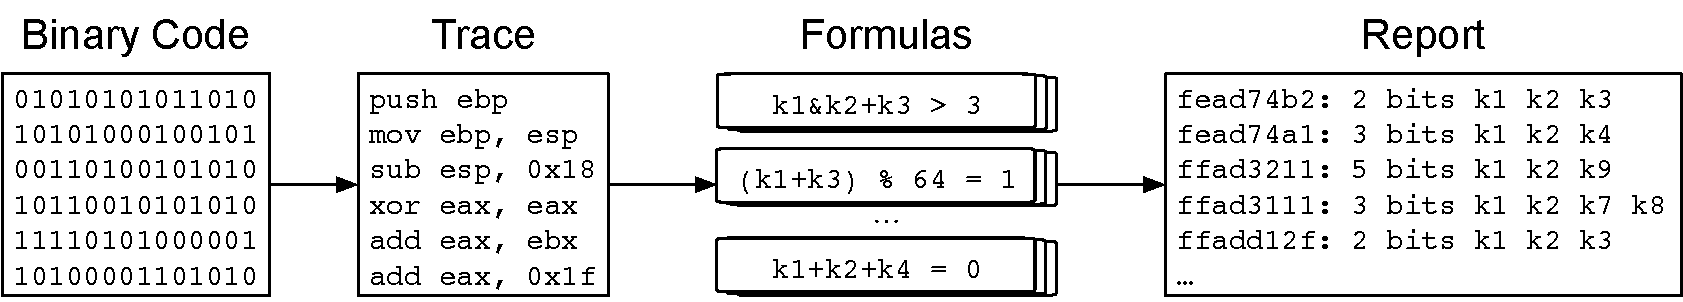
\includegraphics[width=0.85\textwidth]{./figures/chapter4/workflow.pdf}
    \caption{The workflow of \tool{}.}
    \label{fig:workflow}
\end{figure}

\subsection{Execution trace generation} The design goal of \tool{} is to estimate the information leakage as precisely as possible.
We run the target binary under a dynamic binary instrumentation (DBI) tool
to record execution traces and runtime information.
Once the sensitive information is loaded into memory, we start to collect the trace.
In this step, we mark variables and buffers that hold the sensitive data by either annotating the source code (\textsf{make\_abacus\_symbolic}) or telling the DBI tool of the memory address and the length of secrets.

\subsection{Instruction level symbolic execution} We model attackers'
observations from side-channel vulnerabilities with logic formulas.
Each formula captures the fine-grained information between input
secrets and leakage sites. The engine only symbolically executes
instruction that might be affected by the input sensitive data. \tool{} works on one path at a time. The memory model is conceptually similar to other offline executors (e.g., SAGE~\cite{godefroid2008automated} and the trace-based executor of BitBlaze~\cite{song2008bitblaze}). That is, we use symbolic execution to track secrets. When secrets are loaded into the memory, \tool{} starts to interpret instructions symbolically. We treat secrets as symbols ($S$). For other variables, we use concrete values ($C$)
from the execution. We do not know which instruction may manipulate a secret until we execute it. For each instruction, if all its operands and implicit memory accesses are concrete values, we perform concrete calculation and update the destination with the concrete value according to the instruction semantics. Otherwise, we symbolically interpret the instruction and update the destination with a formula.

\subsection{Leakage estimation} We change the information leakage
quantification problem into the counting problem. We propose a
Monte Carlo method to estimate the number of satisfying solutions.
With the help of the Central Limit Theorem (CLT), we also give an error
estimate with the probability, which provides us with the \emph{precision guarantee}.

\tool{} consists of 16,729 lines of code in C++17 and Python. It has three
components: an Intel Pin tool that collects the execution trace, the
instruction-level symbolic execution engine, and the back-end that estimates
the information leakage.

\begin{table}[h!]
    \centering
    %    \resizebox{.8\columnwidth}{!}{
    \caption{\tool{}' main components and sizes}\label{tbl:implementation}
    \begin{tabular}{lr@{~}@{}l}
        \hline
        Component            & \multicolumn{2}{c}{Lines of Code (LOC)}             \\ \hline
        Trace Logging        & 501 lines                               & of C++    \\
        Symbolic Execution   & 14,963 lines                            & of C++    \\
        Data Flow            & 451 lines                               & of C++    \\
        Monte Carlo Sampling & 603 lines                               & of C++    \\
        Others               & 211 lines                               & of Python \\ \hline
        Total                & 16,729 lines                            &           \\\hline
    \end{tabular}
    %    }
\end{table}

Our current implementation supports most Intel 32-bit instructions that are essential to find address-based side-channel
vulnerabilities, including bitwise operations, control transfer, data movement, and logic
instructions. The tool uses the real values to update the registers and memory for instructions that the implementation does not support.
Therefore, the tool may miss some leakages but will not raise false positives.

\section{Evaluation}
\begin{table}[]
    \centering\small\footnotesize
    \caption{Evaluation results overview: Name, Side-channel Leaks\,(Leaks),
        Secret-dependent Control-flows\,(CF), Secret-dependent Data-flows\,(DF),
        The number of instructions\,(\# Instructions), Symbolic Execution\,(SE) and Monte Carlo\,(MC) time.
    }\label{table:over_result}

    %    \resizebox{1.9\columnwidth}{!}{
    \begin{threeparttable}
        \begin{tabular}{l@{}r@{~~}rrr@{~~}rr}
            \hline
            \textbf{Name}     & \textbf{\# Leaks}        & \textbf{\# CF} & \textbf{\# DF}
                              & \textbf{\# Instructions} & \textbf{SE}    & \textbf{MC}                                      \\\hline
                              &                          &                &                &             & ms      & ms      \\\cline{6-7}
            AES\tnote{1}      & 68                       & 0              & 68             & 39,855      & 512     & 1,052   \\
            AES\tnote{2}      & 68                       & 0              & 68             & 39,855      & 520     & 1,057   \\
            AES\tnote{4}      & 75                       & 0              & 75             & 1,704       & 231     & 9,199   \\
            AES\tnote{5}      & 88                       & 0              & 88             & 1,350       & 36      & 1,924   \\
            AES\tnote{6}      & 88                       & 0              & 88             & 1,350       & 35      & 1,961   \\
            AES\tnote{7}      & 88                       & 0              & 88             & 1,420       & 36      & 2,161   \\
            AES\tnote{8}      & 88                       & 0              & 88             & 1,586       & 43      & 1,631   \\
            DES\tnote{1}      & 15                       & 0              & 15             & 4,596       & 58      & 162     \\
            DES\tnote{2}      & 15                       & 0              & 15             & 4,596       & 57      & 162     \\
            DES\tnote{4}      & 6                        & 0              & 6              & 2,976       & 163     & 4,677   \\
            DES\tnote{5}      & 8                        & 0              & 8              & 2,593       & 166     & 6,509   \\
            DES\tnote{6}      & 8                        & 0              & 8              & 2,593       & 165     & 5,975   \\
            DES\tnote{7}      & 8                        & 0              & 8              & 4,260       & 182     & 5,292   \\
            DES\tnote{8}      & 6                        & 0              & 6              & 8,272       & 229     & 5,152   \\
                              &                          &                &                &             & seconds & seconds \\\cline{6-7}
            Chacha20\tnote{3} & 0                        & 0              & 0              & 149,353     & 2       & 0       \\
            Poly1305\tnote{3} & 0                        & 0              & 0              & 1,213,937   & 15      & 0       \\
            Argon2i\tnote{3}  & 0                        & 0              & 0              & 4,595,142   & 37      & 0       \\
            Ed25519\tnote{3}  & 0                        & 0              & 0              & 5,713,619   & 271     & 0       \\
            ECDSA\tnote{1}    & 6                        & 6              & 0              & 4,214,946   & 48      & 31      \\
            ECDSA\tnote{2}    & 4                        & 4              & 0              & 4,192,558   & 102     & 1639    \\
            ECDSA\tnote{5}    & 5                        & 4              & 1              & 8,248,322   & 101     & 62      \\
            ECDSA\tnote{6}    & 5                        & 4              & 1              & 8,263,599   & 100     & 58      \\
            ECDSA\tnote{7}    & 5                        & 4              & 1              & 6,100,465   & 76      & 42      \\
            ECDSA\tnote{8}    & 0                        & 0              & 0              & 10,244,076  & 121     & 0       \\
            ECDSA\tnote{9}    & 0                        & 0              & 0              & 9,266,191   & 102     & 59      \\


                              &                          &                &                &             & minutes & minutes \\\cline{6-7}
            RSA\tnote{1}      & 6                        & 6              & 0              & 22,109,246  & 39      & 41      \\
            RSA\tnote{2}      & 12                       & 12             & 0              & 24,484,441  & 44      & 251     \\
            RSA\tnote{4}      & 107                      & 105            & 2              & 17,002,523  & 23      & 428     \\
            RSA\tnote{5}      & 38                       & 27             & 11             & 14,468,307  & 29      & 436     \\
            RSA\tnote{6}      & 36                       & 27             & 9              & 15,285,210  & 40      & 714     \\
            RSA\tnote{7}      & 31                       & 22             & 9              & 16,390,750  & 34      & 490     \\
            RSA\tnote{8}      & 4                        & 4              & 0              & 18,207,016  & 8       & 53      \\
            RSA\tnote{9}      & 8                        & 8              & 0              & 18,536,796  & 5       & 780     \\
            RSA\tnote{10}     & 11                       & 9              & 2              & 9,527,231   & 2       & 38      \\
            RSA\tnote{11}     & 14                       & 14             & 0              & 10,513,606  & 14      & 503     \\
            RSA\tnote{12}     & 8                        & 8              & 0              & 27,407,986  & 113     & 6560    \\

            Total             & 904                      & 241            & 663            & 167,141,947 & 341m    & 10,232m \\\hline
        \end{tabular}
    \end{threeparttable}
    \begin{tablenotes}
        \scriptsize

        \item[1] mbedTLS\,2.5  ~~~~\item[2] mbedTLS\,2.15 ~\item[3] Monocypher\,3.0 \\
        \item[4] OpenSSL\,0.9.7  ~~\item[5] OpenSSL\,1.0.2f  \item[6] OpenSSL\,1.0.2k \\
        \item[7] OpenSSL\,1.1.0f ~\item[8] OpenSSL\,1.1.1 ~\item[9] OpenSSL\,1.1.1g \\
        \item[10] Libgcrypt\,1.6.1 \item[11] Libgcrypt\,1.7.3 \item[12] Libgcrypt\,1.8.5\\
    \end{tablenotes}
    \vspace*{-20pt}

\end{table}

\subsection{Case Studies}

\subsubsection{Symmetric Ciphers: DES and AES}\label{eval:sym}
We test both DES and AES ciphers from mbedTLS and OpenSSL\@. Both cipher
implementations apply lookup tables, which improve performance but can also introduce side-channels as well. During our evaluation, we find mbedTLS 2.5 and 2.15.1 have the same implementation of AES and DES\@. Therefore, our tool reports the same leakages for both versions.

We find that the DES implementations in both mbedTLS and OpenSSL have several
severe information leakages in the key schedule function.
We do not see any mitigation
in the new version. We think it is not seen as worth the engineering
efforts given the life cycles of DES\@.

\tool{} shows that the AES in OpenSSL 1.1.1 has less leakage than other versions.
OpenSSL 1.1.1 uses 1KB lookup tables with 8-bit entries, unlike older versions that use a table with 32-bit entries. Our tool suggests a smaller lookup table might mitigate side-channel vulnerabilities.

\subsubsection{Monocypher}\label{eval:mono}
Monocypher is a small, easy to use cryptographic library with
performance comparable to LibSodium~\cite{libsodium} and NaCl~\cite{bernstein2012security}.
We choose four ciphers that are
designed to be side-channel resistant from the library.
Because those ciphers have no
data flow from secrets to branch conditions and load addresses.
Monocypher should be safe under our threat models.
We analyze those ciphers with \tool{}, and it reports no leaks.
This indicates that \tool{} is effective for validating countermeasures.

\section{Discussion}
While recent work found many side-channel vulnerabilities,
we note that many of them have not been patched by developers.
Side-channels are ubiquitous in software and it would be difficult to fix all of them.
We need a tool that estimates the sensitivity of each vulnerability
so software engineers can focus on
``severe'' leakages. For example, \tool{} reports that
the modular exponentiation using square and multiply algorithms can
leak more information than a key validation function.

Software developers can use \tool{} to find severe vulnerabilities
and reason about countermeasures.
\tool{} estimates the amount of leaked information for each side-channel leakage
in one execution trace. \tool{} is useful for software
engineers to test programs and fix vulnerabilities.
The design, which is more precise in reporting true leakages as compared with other static
methods~\cite{197207,BacelarAlmeida:2013:FVS:2483313.2483334}, obviously misses
leakages on unexplored traces. The amount of leaked information also depends on the secret key.
However, as the tool is intended for debugging and testing,
we think it is a software engineer's responsibility to select the input key and trigger
the path in which they are interested. It is not a problem for crypto software
since virtually all keys follow similar computational paths.

We use the amount of leaked information to represent the sensitivity level of
each side-channel vulnerability. Although imperfect, \tool{} produces a reasonable
measurement for each leak. For example, the simple modular exponentiation is
notoriously famous for multiple side-channel attacks~\cite{kocher1996timing}.
During the execution, a single leak point may execute multiple times
and each time leak a different bit. In this case, \tool{} reports that the
vulnerability can leak the whole key. However, not every leak point inside a
loop is severe. If a site in the loop leaks the same bit from the
original key, and these leaks are not independent. \tool{} captures most
fine-grained information by modeling each leak during the execution as a
formula and the conjunction of the formulas to describe its total effect.
Some leakage sites (e.g., square and multiply)
can leak one particular bit of the original key, but some leakage sites leak one bit
from several bytes in the original key. \tool{} can capture the dependency among the leaks and
reports more precise leakage information.

\tool{} reaches full precision if the number of estimated leaked bits
equals to Definition~\ref{def}.
\tool{} may lose precision from the
memory model it uses in theory. However, we did not find false positives
caused by the imprecise memory model during our evaluation.
Sampling introduces imprecision but with a probabilistic guarantee.
However, during the evaluation, we find that \tool{} cannot estimate
the amount of leakage for some leakage sites in a reasonable time,
which means the number of $K^o$ is very small. According to Definition~\ref{def},
it means the leakage is very severe. The sampling method in \S\ref{sec:scala} seems
simple and may miss some leakages (e.g., chosen ciphertext attacks) in theory.
However, the evaluation result
shows \tool{} can identify all leakages found by the previous work~\cite{203878,236338,Brotzman19Casym}.